\documentclass[a4paper, 11pt]{article}

\usepackage[utf8]{inputenc} % Encodage des sources
\usepackage[frenchb]{babel} % Typographie francaise
\usepackage[T1]{fontenc} % Pour la police
\usepackage{lmodern} % Pour la police
\usepackage{titling} % Pour récupérer les info de la page de titre
\usepackage[plain]{fullpage} % Utilisation de toute la page
\usepackage{color} % Couleur
\usepackage{graphicx} % Images
\usepackage{hyperref} % Liens
\hypersetup{
	colorlinks,
	citecolor=blue,
	filecolor=black,
	linkcolor=blue,
	urlcolor=blue
}

\usepackage{listings} % Codes
\lstset{
frame=single,
frameround=tttt,
keywordstyle=\bfseries \ttfamily \color{blue},
commentstyle=\color[rgb]{0.133,0.545,0.133},
stringstyle=\ttfamily \color{red},
showstringspaces=true,
tabsize=4,
basicstyle=\footnotesize \ttfamily,
numberstyle=\footnotesize \ttfamily,
numbers=left,
breaklines=true,
breakatwhitespace=true,
aboveskip={\baselineskip},
belowskip={\baselineskip},
columns=fixed,
extendedchars=true,
} 

%% Personnalisation du pied de page et de l'en-tete %%
\usepackage{fancyhdr}
\pagestyle{fancy}
\lhead{}
\chead{}
\rhead{}
\renewcommand{\headrulewidth}{0pt}
\lfoot{\thetitle}
\cfoot{}
\rfoot{\thepage}
\renewcommand{\footrulewidth}{0.4pt}

%% Parametre du titre perso %%
\title{PVETE - Projet de VEille TEchnologique \\
Vers une carte d'identité des langages de programmation}
\author{{\sc Joubert} Sylvain \hspace{1cm} {\sc Mignot} Philippe}
\date{Novembre 2010 - Mars 2011}

\begin{document} %%%%%%%%%%%%%%%%%%%%%%%%%%%%%%%%%%%%%%%%%%%%%%%%%%%%%%%%

%% Titre %%
\begin{titlepage}
\begin{center}
\LARGE \thetitle \normalsize \\
\bigskip \bigskip \bigskip
\large \theauthor \\
\bigskip \bigskip
\thedate \normalsize
\end{center}

\vspace*{\fill}

\begin{center}
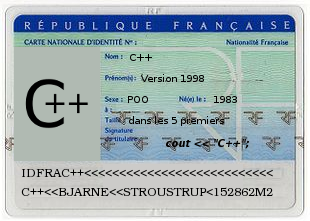
\includegraphics[scale=1.2]{img/carte.png}
\end{center}

\vspace*{\fill}
\vspace*{\fill}


\includegraphics[scale=1]{img/cc}\\
Œuvre mise à disposition selon les termes de la \href{http://creativecommons.org/licenses/by-nc-sa/3.0/}{Licence Creative Commons BY-NC-SA 3.0}
\end{titlepage}

%% Sommaire %%
\tableofcontents
\newpage

%% Texte %%
\section{Introduction}

\subsection{Problématique}
Si parmi les développeurs une grande majorité sait par exemple que le Java et le C++ sont des langages objets et sont parfois capables d'en citer d'autres, un nombre beaucoup plus réduit est capable de citer des langages réflexifs, fonctionnels, à programmation par contrat, …
Et pour cause, il faut déjà savoir de quoi il s'agit.\\

C'est entre autre dans cette optique que se situe ce projet de veille technologique : décrire ce qu'est un langage de programmation via ses caractéristiques.
Le but final est de construire ce que l'on pourrait appeler une carte d'identité des langages de programmation, à savoir un squelette regroupant des caractéristiques (techniques notamment) comme, par exemple, le type du code objet (s'agit-il de binaire, de byte-code ou directement des sources).
Chaque langage est ainsi spécifique de par son agrégation de notions. Il s'agit donc de décrypter l'ADN des langages de programmation.\\

De plus, même si ce n'est pas l'objectif de ce projet, une fois cette carte d'identité construite cela pourrait permettre de générer une base de données des langages et d'y effectuer des recherches simplement et efficacement.
En effet, comment feriez-vous aujourd'hui pour savoir quels sont les langages objets, réflexifs, compilés et supportant la généricité du code ?

\subsection{Contexte}

\subsubsection{Langage informatique}

Un langage est constitué d’un ensemble de signes doté d’une sémantique, et le plus souvent d’une syntaxe. Contrairement aux langages naturels, qui sont destinés à la communication entre les humains, les langages informatiques ont pour but de décrire l’ensemble des actions consécutives qu’une machine doit effectuer. Les protocoles de communication, qui servent à la communication entre les machines, ne sont donc pas considérés comme des langages informatiques.\\

Un langage informatique a pour but originel la conception, la mise en œuvre ou l’exploitation d’un système d’information. Néanmoins, ils sont également utilisés pour effectuer d’autres tâches, comme la maintenance du système d’information, la création d’interface graphique, la programmation de commandes numériques, la statistique, etc. Les langages de conception (UML, Merise, …), les langages de structuration de contenu (HTML, XML, tous les langages de balisage en général), les méthodes formelles, les langages de définition de données et les langages de requêtes (SQL, …) sont des langages informatiques, ainsi que, bien sûr, les langages de programmation.\\

Ce type de langage est destiné à la fois à la machine et à l’humain. En effet, les instructions contenues dans le code correspondent à des actions que doit effectuer le processeur. \cite{bib_infoclick} En outre, le code doit pouvoir être écrit et compris par les humains. Le langage utilisé par le processeur est le langage machine, constitué de données binaires. Pour que le processeur exécute les instructions définies dans le code du langage informatique, il faut d’abord le transformer en langage machine.

\subsubsection{Langage de programmation}

Un langage de programmation fournit une abstraction de niveau supérieur pour utiliser une machine, car très peu d’humains comprennent le langage machine. La notion de programme est apparue au cours de la deuxième moitié du XIXème siècle, mais les premiers langages de programmation datent des environs de l’année 1950. Dans les années 60, de nombreux langages spécialisés sont créés. Les langages dits généraux commencent à s’imposer à partir des années 70 (langage C et Pascal). Les langages orientés objet apparaissent dans les années 80. Vers 1990 arrivent les langages Java, Perl et Python. \cite{bib_knuth} La programmation Internet apparaît dans les années 2000.\\

Étant donné que tout le monde peut créer son propre langage de programmation, il est impossible d’estimer le nombre total de langages de programmation avec précision, mais il est sûr que ce nombre est de l’ordre de quelques milliers. \cite{bib_scriptol} \cite{bib_dowek} La transformation du code source d’un langage de programmation en langage machine peut se faire de différentes façons. En premier lieu, le code peut être interprété par un logiciel interpréteur, qui va lire chaque ligne du code au cours de l’exécution du programme, et envoyer l’instruction correspondante au processeur sous forme binaire. En second lieu, le code peut être transformé directement sous forme exécutable par un compilateur. Cette solution permet une meilleure performance, parce que le programme est compilé une bonne fois pour toutes. Cependant, elle nécessite de recompiler le code source à chaque modification. Elle garantit également la sécurité du code source, car le programme ainsi diffusé est en langage machine.\\

Une fois défini ce que l’on entend exactement par langage de programmation on se permettra d’utiliser l’expression «langage» seule pour «langage de programmation».

\subsubsection{Organisation de la suite de l'étude}

La suite de ce rapport sera organisée de la façon suivante :
\begin{itemize}
\item résultat de l'étude : une carte d'identité des langages de programmation,
\item présentation des différentes caractéristiques de la carte d'identité,
\item proposition de quelques exemples.\\
\end{itemize}

\section{Caractéristiques d'un langage}

\subsection{Carte d'identité}

Le résultat de l'étude se résume à la carte d'identité suivante :\\

\renewcommand{\labelitemi}{\textbullet}
\begin{itemize}
\item \hyperref[generalites]{Généralités}
	\begin{itemize}
	\item \hyperref[nom]{nom}
	\item \hyperref[version]{version}
	\item \hyperref[date_creation]{date de création}
	\item \hyperref[createur]{créateur(s)}
	\item \hyperref[logo]{logo}\\
	\end{itemize}
\item \hyperref[paradigmes]{Paradigmes}
	\begin{itemize}
	\item impératif
	\item fonctionnel
	\item orienté objet
	\item …\\
	\end{itemize}
\item \hyperref[typage]{Typage}
	\begin{itemize}
	\item \hyperref[fort_faible]{fort | faible}
	\item \hyperref[statique_dynamique]{statique | dynamique}
	\item \hyperref[explicite_implicite]{explicite | implicite}\\
	\end{itemize}
\item \hyperref[divers]{Divers}
	\begin{itemize}
	\item \hyperref[turing]{turing-complétude}
	\item \hyperref[evaluation]{évaluation}
	\item \hyperref[memoire]{gestion de la mémoire}\\
	\end{itemize}
\item \hyperref[communaute]{Communauté}
	\begin{itemize}
	\item \hyperref[popularite]{popularité}
	\item \hyperref[implementations]{implémentations}\\
	\end{itemize}
\item \hyperref[code]{Code}
	\begin{itemize}
	\item \hyperref[objet]{code objet}
	\item \hyperref[hello]{Hello world!}\\
	\end{itemize}
\end{itemize}

Les précédentes caractéristiques sont explicitées ci-après.

\subsection{Généralités}
\label{generalites}

\subsubsection{Nom}
\label{nom}

Le nom usuel du langage. Exemples : Prolog, C, Java, …

\subsubsection{Version}
\label{version}

Un langage de programmation possède souvent différentes révisions, au fur et à mesure de son évolution. Les principales méthodes d'appellation de version sont :
\begin{itemize}
\item l'incrémentation du numéro de version (exemples : Java 1.3, 1.4, 5, 6)
\item la date de normalisation (exemples : C89, C90, C99)
\end{itemize}

\subsubsection{Date de création}
\label{date_creation}

La date de création correspond la plupart du temps à la sortie de la première version officielle de la description d'un langage. Exemples : le C est annoncé en 1973, le Python en 1990.

\subsubsection{Créateur(s)}
\label{createur}

Souvent, les spécifications d'un langage sont modifiées et améliorées par la communauté, mais la paternité reste à celui qui a proposé la première version. Il arrive parfois que le créateur d'un langage soit une entreprise. Exemples : Bjarne Stroustrup a créé le C++, 	Dennis Ritchie le C, Sun Microsystems le Java, Google le Go.

\subsubsection{Logo}
\label{logo}

Certains langages possèdent parfois un logo qui permet de les identifier plus facilement. Cependant, cette pratique reste peu commune une fois ramenée au nombre de langages existants.\\

Exemples :\\

\begin{tabular}{ccc}

\includegraphics[scale=0.4]{img/java} &

\includegraphics[scale=0.5]{img/python} &
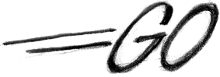
\includegraphics[scale=0.8]{img/go}\\
Java & Python & Go
\end{tabular}

\subsection{Paradigmes}
\label{paradigmes}

\subsubsection{Définition}

Après un minimum de recherche, force est de constater que la notion de paradigme revient régulièrement lorsqu’il s’agit de décrire un langage de programmation.
De manière générale un paradigme est un mode de représentation d’une réalité quelconque. C’est une manière structurée de voir et de concevoir. Ainsi, un paradigme de programmation est une manière de penser, d’écrire et de structurer un programme et donc par extension son code source. Le code source étant lui-même régit par la syntaxe du langage utilisé, on retombe effectivement sur le fait qu’un langage est particulièrement caractérisé par son (ou ses) paradigme(s) de programmation.\\

Les paradigmes de programmation sont très nombreux et à un langage ne correspond pas un unique paradigme. La plupart du temps un langage autorise plusieurs paradigmes voire des paradigmes «dégénérés» dans le sens où toutes les fonctionalité de ces derniers ne sont pas forcément présente dans le langage. Tout ceci rend l’affectation de paradigme à un langage particulièrement ardue et semble être une part importante du travail qu’il nous reste à faire dans l’élaboration de notre carte d’identité.
À titre d’exemple et parmis les plus connus, citons la programmation orientée objet qui visualise un programme comme un assemblage d’entités (objets) communiquant entre elles, la programmation fonctionnelle où la base du code est la fonction (au sens mathématique du terme). Parmis les moins utilisés citons la programmation par contrainte ou la programmation par contrat.

\subsubsection{Tour d'horizon}

Il existe un grand nombre de paradigmes de programmation (plusieurs dizaines). Certains sont d'ailleurs surement restés inconnus. Le premier d'entre eux et le plus courant, celui dont les premiers langages de programmation se sont inspirés, est la programmation impérative. Ce paradigme décrit les opérations en termes de séquences d'instructions exécutées par l'ordinateur pour modifier l'état d'un programme. La plupart des processeurs fabriqués aujourd'hui fonctionnent sur ce principe. Par la suite, de nombreux langages de programmation se sont développés et ont implémentés de plus en plus de paradigmes différents \cite{bib_levenez}, \cite{bib_mandriva}. Il existe des tentatives de classification des différents paradigmes, mais ils sont tellement différents que cela devient vite compliqué \cite{bib_ucl}.\\

Certains paradigmes sont comparables à d'autres, tandis que la plupart ne peuvent pas être classés en catégories. Par exemple, on peut dire que la programmation procédurale est comparable à la programmation fonctionnelle. En effet, la première est basée sur l'appel de procédures (c'est-à-dire des fonctions qui ne renvoient rien), alors que la seconde fait appel à des fonctions mathématiques qui s'envoient des résultats les unes aux autres. De la même manière, la programmation par contrainte est comparable à la programmation logique : elles s'appuient toutes les deux sur des relations que vont avoir les entités entre elles (relation contrainte : une variable va évoluer en fonction d'une autre variable, relation factuelle : un fait va avoir des conséquences).\\

La programmation évènementielle est différente de la programmation séquentielle. L'une est constituée de deux boucles qui récupèrent et qui gèrent les évènements tandis que l'autre exécute toujours les mêmes instructions. Deux différents paradigmes pourraient également être la programmation itérative et la programmation récursive.\\

Pour plus d'informations sur les paradigmes de programmation en général consulter Wikipédia. \cite{bib_wiki_paradigmes}
Il en existe donc une grande panoplie. Pour fixer les idées suit un exemple.

\subsubsection{Un paradigme courant : l'abstraction de données}

La programmation par abstraction de données repose sur une notion principale : les types abstraits de données ou TAD. Il s'agit de regrouper et manipuler les données d'un programme comme des boites noires. \cite{bib_dchaffiol1}, \cite{bib_dchaffiol2}, \cite{bib_wiki_adt}\\

Du point de vue de l'utilisation, les TAD reposent sur deux règles \cite{bib_reunion} :
\begin{itemize}
\item déclarer un type de données représentant un concept
\item définir le comportement de ce type de données et les manipulations possibles sur celui-ci\\
\end{itemize}

En revanche, la définition d'un TAD n'est jamais connue d'un utilisateur (ou du moins n'a pas besoin d'être connue).\\

Prenons par exemple un TAD présent dans la bibliothèque standard du langage C : FILE.
Tout programmeur C a déjà vu et utilisé ce type. Il s'agit en effet d'un TAD :
\begin{itemize}
\item on sait qu'il existe un type FILE représentant un fichier mémoire
\item on connait son comportement : il se comporte de manière à permettre un accès aux données d'un fichier et surtout on sait manipuler ce type (via des fonctions en C comme fopen, fclose, fprintf, …)\\
\end{itemize}

En revanche, personne n'a à savoir comment est défini FILE pour pouvoir l'utiliser. Et d'ailleurs, la définition est quasiment impossible à trouver. Sur ma machine, je n'ai réussi qu'à trouver la déclaration dans stdio.h :

\begin{lstlisting}[language=c]
struct _IO_FILE;
typedef struct _IO_FILE FILE;
\end{lstlisting}

Comme quoi on n'est pas plus avancé.\\

Un TAD n'est pas caractérisé par sa structure mais par son comportement et ses possibilités de manipulation. Dans ce sens, on peut dire que la programmation par abstraction de données est un paradigme parent de la programmation orientée objet. Celle-ci étend encore plus ce concept (via le principe d'encapsulation) et met l'accent sur les liens de communication entre les objets (méthodes) alors que les TAD sont beaucoup plus orientés manipulation. Il existe de nombreuses structures de données utilisées la plupart du temps comme un TAD. Les plus classiques sont les types «fichier» (comme FILE), les piles, les files ou les arbres.\\

Si ce concept de programmation est très largement utilisé, c'est aussi parce de nombreux langages le supportent (ou alors ces langages supportent-ils ce paradigme parce qu'il est très utilisé ?). On a déjà cité le C, il faut ajouter à cela les langages objets (C++, Java, …) et plus généralement l'ensemble des langages permettant au programmeur de définir ses propres types de données (soit une bonne partie des langages existants). \cite{bib_univnc}

\subsection{Typage}
\label{typage}

L'une des premières choses que l'on apprend dans un langage de programmation (après le classique Hello world!) est l'utilisation des variables. Pour le sujet qui nous intéresse les variables nous mènent à leur type et à ce qu'on appelle le typage d'un langage. Celui-ci possède généralement trois caractéristiques. \cite{bib_wiki_typage}

\subsubsection{Fort | faible}
\label{fort_faible}

Cette notion est la plus floue des trois caractéristiques car personne n'a encore été en mesure d'en proposer une définition précise et communément admise. Cette notion regroupe entre autres la capacité du compilateur à déterminer à la compilation et/ou à l'exécution les erreurs de typage (du style affectation d'une chaîne de caractères dans un entier). Plus cette détection est forte et possible plus le typage est fort. De même, de nombreux langages autorisent par exemple l'affectation d'une valeur d'une variable entière dans une variable flottante. Il s'agit donc plus d'une échelle de valeur que d'une notion binaire. Pour ce qui est des exemples, le C est faible (conversions implicites autorisées) tandis que le Java est fort (cast obligatoire dans 99\% des cas).

\subsubsection{Statique | dynamique}
\label{statique_dynamique}

Pour peu que l'on s'intéresse à la compilation, la différence entre statique et dynamique ne pose pas de problème. Le typage statique est effectué lors de la compilation. Le typage dynamique est lui vérifié et déterminé à l'exécution. Ce dernier est souvent associé à la possibilité pour une variable de changer de type en cours d'exécution. Ainsi en PHP (qui par ailleurs possède un typage implicite), il est tout à fait possible d'écrire le code suivant :

\begin{lstlisting}[language=php]
$var = 42;
$var = "Un elePHPant ca trompe enormement";
\end{lstlisting}

Cependant, comme tout mécanisme dynamique qui se respecte, cela dégrade les performances.

\subsubsection{Explicite | implicite}
\label{explicite_implicite}

Cette caractéristique détermine si le programmeur doit préciser explicitement ou non dans le code source le type d'une variable. Par exemple, si le typage est explicite le code dit clairement «voici une variable a, c'est un entier qui vaut 42». C'est la cas notamment du langage C :

\begin{lstlisting}[language=c]
int a = 42;
\end{lstlisting}

Dans le cas implicite, le code dit plutôt «voici une variable a, sa valeur est l'entier 42». La différence réside dans le fait que le type de a dépend de ce qu'on lui affecte. Par conséquent, si le langage n'a pas de typage dynamique, une déclaration implicite nécessite une initialisation. La plupart des langages à typage implicite utilisent un mécanisme d'inférence de types pour résoudre le type. \cite{bib_wiki_inference} Exemple en Caml :

\begin{lstlisting}[language=caml]
let a = 42;;
\end{lstlisting}

NB : Le C++ jusqu'à aujourd'hui est un langage à typage explicite. Cependant cela devrait changer avec l'arrivée du prochain standard (C++0x/C++1x) et l'introduction du mot-clé 'auto'. \cite{bib_wiki_inference_cpp}

\subsection{Divers}
\label{divers}

\subsubsection{Turing-complétude}
\label{turing}

Le concept de turing-complétude est apparu suite à l'invention de la machine de Turing en 1936 par Alan Turing. Cette invention a donné le coup d'envoi à la création des machines programmables, et donc aux premiers programmes. De nos jours, on qualifie généralement un langage de programmation de turing-complet s'il peut calculer toutes les fonctions calculables. Nous allons voir que la définition de ce concept n'est pas aussi simple… En premier lieu, nous allons définir ce qu'est une machine de Turing. En second lieu, nous verrons comment cette définition est appliquée aux langages de programmation.

\paragraph{La machine de Turing}

Ayant été inventée avant l'ordinateur, elle avait pour but de décrire une personne virtuelle qui était censée exécuter une suite d'opérations sur un tableau infini d'un nombre fini de caractères. La machine de Turing est de ce fait composée des éléments suivants :
\begin{itemize}
\item un «ruban» contenant une infinité (vers la droite et vers la gauche) de cases consécutives dans lesquelles sont stockées des symboles appartenant à un alphabet. En général, cet alphabet contient les deux caractères '0' et '1', le premier étant considéré comme le caractère par défaut, ou «blanc» (ce «blanc» est un caractère de référence présent dans tous les alphabets utilisés dans une machine de Turing)
\item une tête de lecture/écriture qui peut lire et écrire dans une case. Elle peut se déplacer d'une case à la fois, vers la droite ou vers la gauche
\item un registre d'état qui contient l'état courant du système. Il existe toujours un nombre fini d'états. Au début, ce registre contient un «état de départ»
\item une table d'actions composée des différentes instructions décrivant à la machine quel symbole écrire, comment déplacer la tête de lecture (vers la gauche ou vers la droite), et quel est le nouvel état, en fonction de ce que contient la case lue et de l'état précédent. S'il n'y a plus d'actions dans la table, c'est que le programme est terminé\\
\end{itemize}

\begin{center}
\begin{tabular}{c}
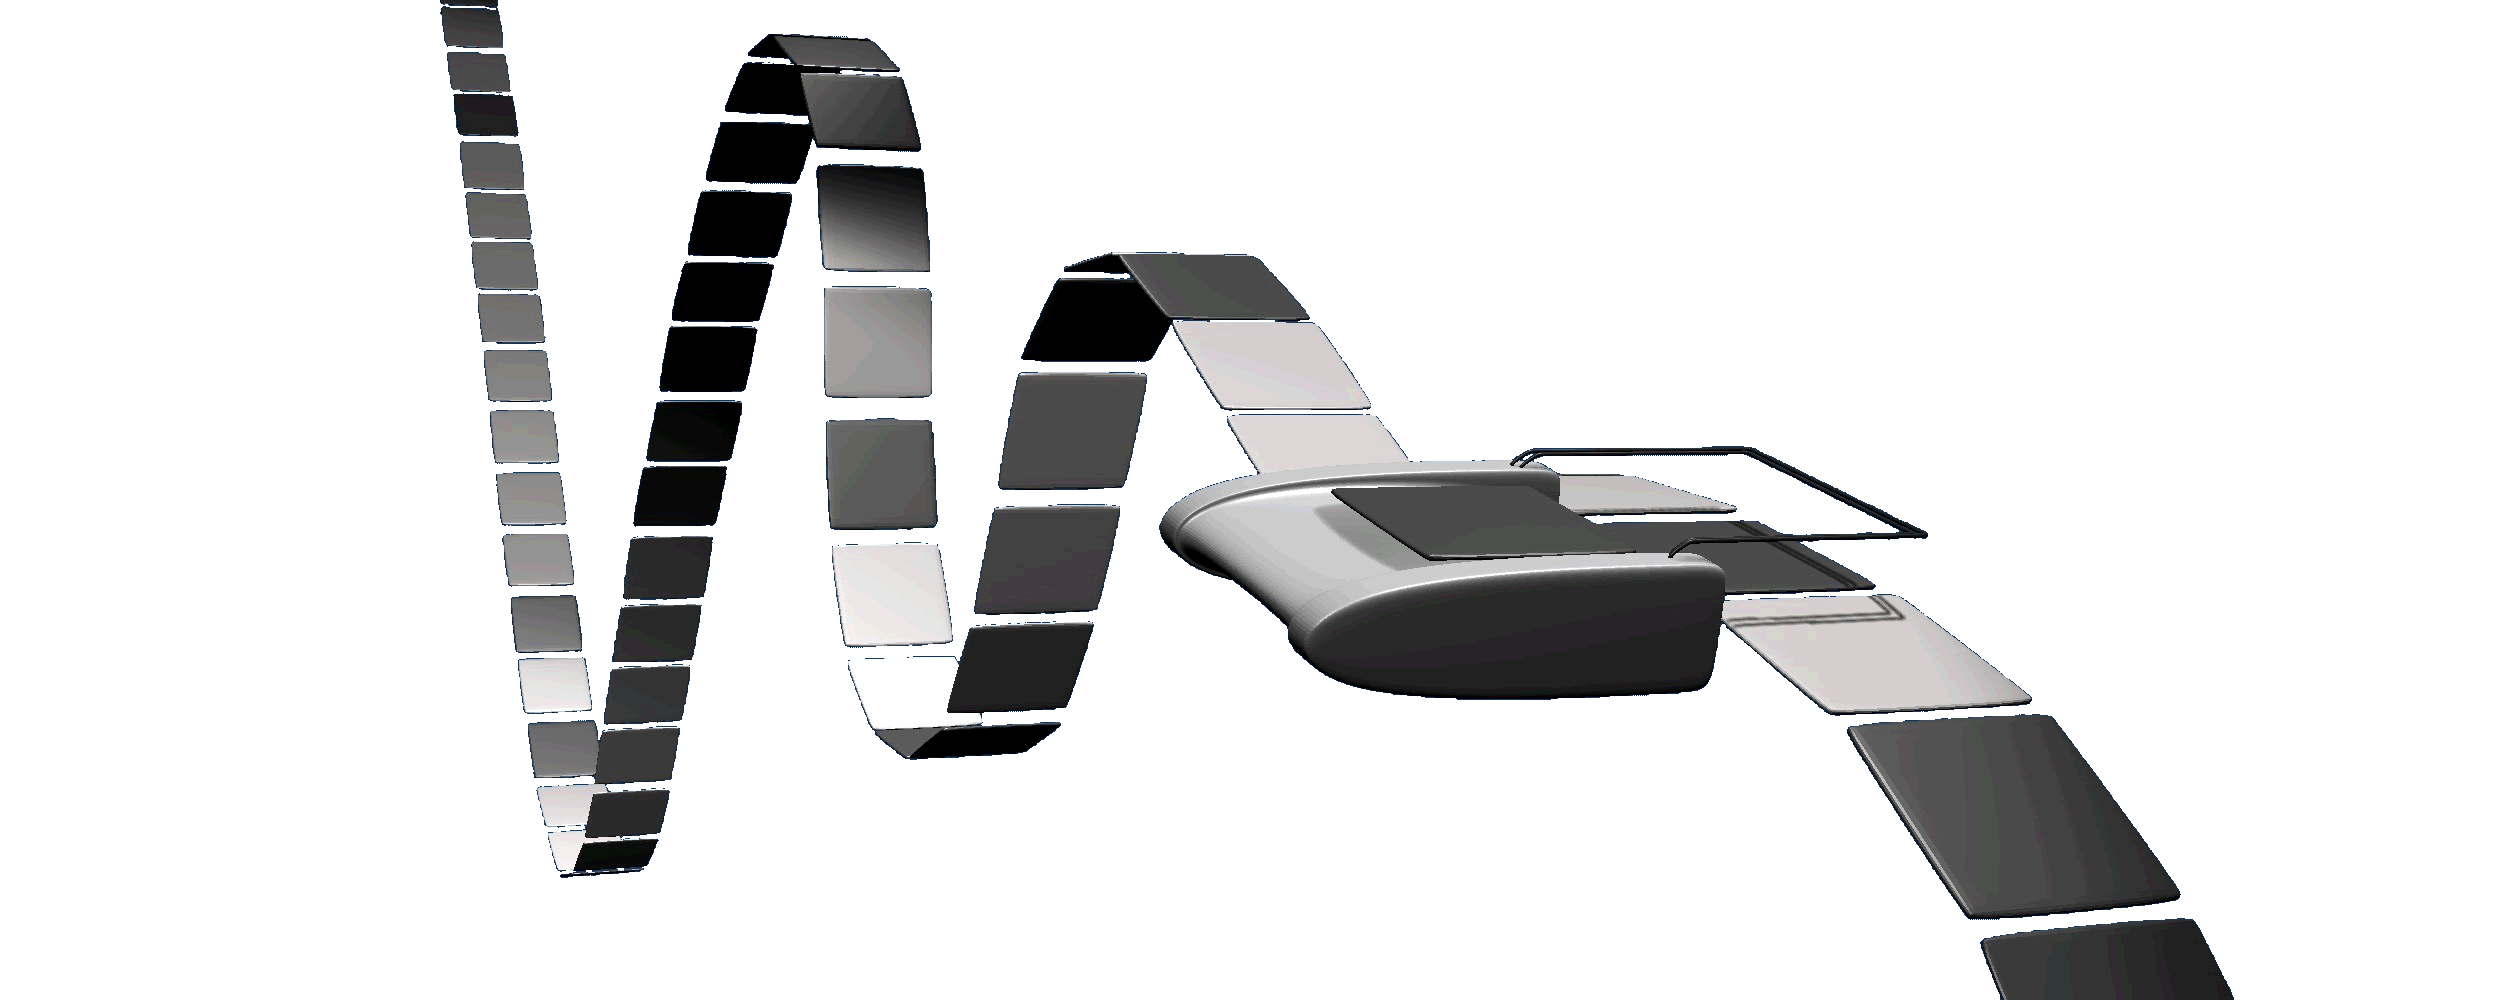
\includegraphics[scale=0.15]{img/turing}\\
Représentation imagée d'une machine de Turing
\end{tabular}
\end{center}

En pratique, voici comment se comporte une machine de Turing \cite{bib_wiki_turing} \cite{bib_jdn} :
\begin{enumerate}
\item lire le symbole qui se trouve dans la case où est située la tête de lecture
\item suivant l'état courant et la valeur lue, écrire une nouvelle valeur dans cette case et déplacer la tête de lecture vers la droite ou vers la gauche
\item enregistrer le nouvel état du système, puis reprendre la première étape
\end{enumerate}

\paragraph{Application aux langages de programmation}

On dit d'un langage de programmation qu'il est turing-complet quand il permet de représenter toutes les fonctions calculables au sens de Turing et Church. \cite{bib_w3support} \cite{bib_wiki_lambda} En pratique, il faut que le langage permette d'émuler une machine de Turing, ou une autre machine turing-complète. En général, les langages turing-complets comprennent les possibilités suivantes :
\begin{itemize}
\item l'allocation dynamique de mémoire
\item la récursivité ou un autre moyen d'exécuter des boucles infinies
\item l'exécution infinie (pas de garantie de fin de programme)
\item le lambda-calcul (défini par Alonzo Church en 1930)\\
\end{itemize}

La turing-complétude n'apporte pas de «pouvoir» supplémentaire à un langage de programmation. En effet, certains langages faits pour une application spécifique ne sont pas turing-complets et n'ont pas besoin de l'être. Cette notion signifie juste que le langage peut être utilisé pour calculer tout ce que l'on veut. Par exemple, le langage SQL n'est devenu turing-complet qu'en 1999 (avec la récursivité), mais à l'époque il suffisait amplement à ce qu'il était censé faire. Les langages «usuels», comme le Java, le C ou le C++ sont en général turing-complet. Des langages très basiques peuvent également être turing-complets (exemple : le Brainfuck).\\

Il faut préciser que le terme «turing-complet» n'est pas tout à fait exact, car la mémoire d'une machine ne peut pas être infinie alors qu'une machine de Turing possède un ruban de taille infinie. Cependant, étant donné qu'une telle machine ne peut pas exister, un abus de langage s'est créé.

\subsubsection{Évaluation}
\label{evaluation}

Cette notion définit la méthode d'évaluation des expressions. Il existe deux stratégies d'évaluation :
\begin{itemize}
\item l'évaluation stricte : l'expression est évaluée au plus tôt
\item l'évaluation paresseuse : l'expression est évaluée lorsqu'on a besoin de sa valeur\\
\end{itemize}

La plupart des langages de programmation utilisent l'évaluation stricte.

\subsubsection{Gestion de la mémoire}
\label{memoire}

Elle peut être de deux sortes :
\begin{itemize}
\item la gestion de la mémoire est laissée aux soins de l'utilisateur, exemple : les fonctions malloc et free en C
\item la gestion de la mémoire est gérée par l'implémentation du langage, exemple : le «garbage collector» de la machine virtuelle de Java
\end{itemize}

\subsection{Communauté}
\label{communaute}

\subsubsection{Popularité}
\label{popularite}

Il est très difficile de mesurer objectivement la popularité d'un langage faute de définition précise. On peut cependant envisager de prendre en compte :
\begin{itemize}
\item le nombre de ligne de code en production
\item le nombre de personnes «sachant programmer»
\item le nombre d'offres d'emploi pour ce langage
\item le nombre de livres vendus
\item …\\
\end{itemize}

On pourrait envisager une classification simple mais difficile à préciser :
\begin{itemize}
\item langages populaires (C, C++, Java, …)
\item langages secondaires
\item langages marginaux (nouveaux langages ou langages qui n'ont pas trouvé de public)
\item langages exotiques (Brainfuck et Whitespace)\\
\end{itemize}

Tiobe \cite{bib_tiobe} est un site qui présente un classement des langages les plus populaires, ainsi que leur évolution.
Langpop \cite{bib_langpop} semble aussi être un bon site de résultats. Il a en tout cas le mérite d'avoir de nombreuses sources différentes.

\subsubsection{Implémentations}
\label{implementations}

Une implémentation d'un langage est un moyen utilisé par l'ordinateur de lire le code source et de permettre son exécution en générant du code machine. La plupart du temps, il s'agit soit d'un compilateur, soit d'un interpréteur. Exemple : gcc et le compilateur de Microsoft Visual Studio sont des implémentations différentes du C. \cite{bib_compl}

\subsection{Code}
\label{code}

\subsubsection{Code objet}
\label{objet}

Un signe caractéristique d'un langage est ce que l'on pourrait appeler la nature de son code objet :
\begin{itemize}
\item le langage peut être compilé (C, C++, …), dans ce cas le code objet est du binaire
\item il peut être interprété pur (PHP, Ruby, Perl et tous les langages de scripts), dans ce cas le code objet est également le code source
\item finalement, le mélange des deux existe aussi (Java par exemple), dans ce cas le code source est compilé en byte-code et ce dernier est interprété, le code objet est donc du byte-code
\end{itemize}

\subsubsection{Hello world!}
\label{hello}

Le Hello world! correspond à un code minimal d'exemple, consistant en l'affichage de la phrase «Hello world!» sur la sortie standard. Il est intéressant d'inclure des commentaires dans le code source du Hello world!, puisque ceux-ci font partie intégrante de la syntaxe du langage.
\section{Cartes d'identités}

\subsection{Python}

\begin{figure}[!ht]
	\center
	
\includegraphics[scale=0.4]{img/python.jpeg}
\end{figure}

\renewcommand{\labelitemi}{\textbullet}
\begin{itemize}
\item Généralités
	\begin{itemize}
	\item nom : Python
	\item version : 3.2 (sortie en 2011)
	\item date de création : 1990
	\item créateur : Guido van Rossum\\
	\end{itemize}
\item Paradigmes
	\begin{itemize}
	\item impératif
	\item orienté objet
	\item fonctionnel
	\item réflexif\\
	\end{itemize}
\item Typage
	\begin{itemize}
	\item fort
	\item dynamique
	\item implicite\\
	\end{itemize}
\item Divers
	\begin{itemize}
	\item turing-complétude : oui
	\item évaluation : stricte
	\item gestion de la mémoire : à la charge de l'implémentation\\
	\end{itemize}
\item Communauté
	\begin{itemize}
	\item popularité : langage populaire, parmi les 10 premiers
	\item implémentations : CPython, Jython, IronPython, PyPy\\
	\end{itemize}
\item Code
	\begin{itemize}
	\item code objet : principalement le code source mais du byte code peut aussi être généré
	\item Hello world! :
\begin{lstlisting}[language=python]
# Affichage standard
print("Hello world!")
\end{lstlisting}
	\end{itemize}
\end{itemize}

\newpage

\subsection{C++}

\begin{figure}[!ht]
	\center
	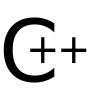
\includegraphics[scale=0.7]{img/cxx}
\end{figure}

\renewcommand{\labelitemi}{\textbullet}
\begin{itemize}
\item Généralités
	\begin{itemize}
	\item nom : C++
	\item version : 2008
	\item date de création : 1983
	\item créateur : Bjarne Stroustrup\\
	\end{itemize}
\item Paradigmes
	\begin{itemize}
	\item générique
	\item orienté objet
	\item procédural
	\item récursif
	\item …\\
	\end{itemize}
\item Typage
	\begin{itemize}
	\item faible
	\item statique
	\item explicite\\
	\end{itemize}
\item Divers
	\begin{itemize}
	\item turing-complétude : oui
	\item évaluation : stricte
	\item gestion de la mémoire : peut être gérée par l'utilisateur\\
	\end{itemize}
\item Communauté
	\begin{itemize}
	\item popularité : langage populaire, parmi les 5 premiers
	\item implémentations : g++, Borland C++ Compiler, Digital Mars, Visual C++, …\\
	\end{itemize}
\item Code
	\begin{itemize}
	\item code objet : code binaire, il s'agit d'un langage compilé
	\item Hello world! :
\begin{lstlisting}[language=c++]
#include <iostream> // Commentaire : utilisation de la sortie standard

int main(void)
{
    /* Commentaire : 'std::' sert a acceder a l'espace de noms std,
       dans lequel sont definies les variables cout et endl. */
    std::cout << "Hello world!" << std::endl;
    return 0;
}
\end{lstlisting}
	\end{itemize}
\end{itemize}

\newpage

\subsection{Prolog}

\renewcommand{\labelitemi}{\textbullet}
\begin{itemize}
\item Généralités
	\begin{itemize}
	\item nom : Prolog (acronyme de PROgrammation LOgique)
	\item version : 2000
	\item date de création : 1972
	\item créateurs : Alain Colmerauer, Philippe Roussel\\
	\end{itemize}
\item Paradigmes
	\begin{itemize}
	\item programmation logique
	\item récursif\\
	\end{itemize}
\item Typage : la qualification du typage du prolog n'a pas vraiment de sens puisqu'il n'existe pas réellement de variables. Cependant, en essayant d'extrapoler sur les mécanismes d'évaluation des valeurs il serait dynamique, fort et implicite\\
\item Divers
	\begin{itemize}
	\item turing-complétude : oui
	\item évaluation : paresseuse\\
	\end{itemize}
\item Communauté
	\begin{itemize}
	\item popularité : langage marginal ($> 30^{ème}$ place)
	\item implémentations : BProlog, GNUProlog, Poplog Prolog, P\#, …\\
	\end{itemize}
\item Code
	\begin{itemize}
	\item code objet : code binaire lorsque les performances comptent, parfois byte code en fonction de l'implémentation
	\item Hello world! :
\begin{lstlisting}[language=prolog]
?- write('Hello world!'), nl
Hello World!
true.
\end{lstlisting}
	\end{itemize}
\end{itemize}

\newpage

\subsection{Java}

\begin{figure}[!ht]
	\center
	
\includegraphics[scale=0.3]{img/java}
\end{figure}

\renewcommand{\labelitemi}{\textbullet}
\begin{itemize}
\item Généralités
	\begin{itemize}
	\item nom : Java
	\item version : 6.0 (sorti en 2006)
	\item date de création : 23 mai 1995
	\item créateur : Sun Microsystem\\
	\end{itemize}
\item Paradigmes
	\begin{itemize}
	\item générique
	\item orienté objet
	\item structuré
	\item impératif
	\item …\\
	\end{itemize}
\item Typage
	\begin{itemize}
	\item fort
	\item statique
	\item explicite\\
	\end{itemize}
\item Divers
	\begin{itemize}
	\item turing-complétude : oui
	\item évaluation : stricte
	\item gestion de la mémoire : gérée par l'implémentation\\
	\end{itemize}
\item Communauté
	\begin{itemize}
	\item popularité : langage populaire, parmi les 5 premiers
	\item implémentations : HotSpot, JamaicaVM, GIJ, OpenJDK, …\\
	\end{itemize}
\item Code
	\begin{itemize}
	\item code objet : byte code
	\item Hello world! :
\begin{lstlisting}[language=java]
// Hello World in Java
class HelloWorld
{
    static public void main(String args[])
    {
        System.out.println("Hello World!");
    }
}
\end{lstlisting}
	\end{itemize}
\end{itemize}

\newpage

\subsection{Brainfuck}

\renewcommand{\labelitemi}{\textbullet}
\begin{itemize}
\item Généralités
	\begin{itemize}
	\item nom : Brainfuck
	\item date de création : 1993
	\item créateur : Urban Müller\\
	\end{itemize}
\item Paradigmes
	\begin{itemize}
	\item à pile\\
	\end{itemize}
\item Typage (même si cela n'a pas beaucoup de sens)
	\begin{itemize}
	\item fort
	\item statique
	\item implicite\\
	\end{itemize}
\item Divers
	\begin{itemize}
	\item turing-complétude : oui
	\item gestion de la mémoire : gérée par l'implémentation\\
	\end{itemize}
\item Communauté
	\begin{itemize}
	\item popularité : langage exotique
	\item implémentations : il en existe une grande quantité vu que chacun peut en coder un facilement du fait de la simplicité du langage\\
	\end{itemize}
\item Code
	\begin{itemize}
	\item code objet : code source, langage interprété
	\item Hello world! :
\begin{lstlisting}
Hello world en Brainfuck
++++++++++[>+++++++>++++++++++>+++>+<<<<-]
>++.>+.+++++++..+++.>++.<<+++++++++++++++.
>.+++.------.--------.>+.>.
\end{lstlisting}
	\end{itemize}
\end{itemize}

\section{Conclusion}

Nos objectifs initiaux étaient d'identifier des caractéristiques communes aux différents langages de programmation afin de les comparer. La carte d'identité résultante de l'étude permet effectivement de réaliser cette comparaison. Les regroupements de caractéristiques ont été fait de la manière la plus cohérente possible, cependant ce n'est sûrement pas la seule façon d'organiser une telle carte d'identité. Les principales caractéristiques y sont présentes bien que l'on puisse probablement en ajouter ou les organiser différemment.\\

La principale difficulté a été de bien cerner les valeurs possibles des caractéristiques. En effet, il s'avère que la plupart d'entre elles ne peuvent pas être remplies de manière objective. Par exemple, la liste des paradigmes supportés par un langage ne peut pas être exhaustive : certains paradigmes ne sont supportés que partiellement, ou sont spécifiques au langage en question. De même, nous avons définis les notions de typages fort | faible, statique | dynamique et explicite | implicite, mais certains langages utilisent un mélange plutôt flou de ces notions. L'exemple le plus frappant de la subjectivité des valeurs des caractéristiques est la mesure de la popularité d'un langage.\\

Ainsi, si l'on voulait réellement construire une base de données pour stocker ces cartes d'identité, il faudrait faire des choix arbitraires quant aux valeurs possibles des caractéristiques. L'étude a permis de se rendre compte que la définition d'une carte d'identité objective et universelle est irréalisable. Cependant, une fois certains choix de conception effectués, il semble tout à fait possible de construire et remplir une bibliothèque des langages de programmation. Une telle base de données permettrait à un programmeur de choisir parmi un panel de langages disponibles celui qui correspond le mieux à ses attentes.\\

Une suite intéressante à ce projet pourrait être l'étude d'une carte similaire en ce qui concerne les autres types de langages : langages de structuration de données, langages de requêtes, …. Et pourquoi pas les langages naturels ?

%\addcontentsline{toc}{section}{Références}
\bibliographystyle{unsrt}
\bibliography{biblio}

\end{document}

